\documentclass[compress,red]{beamer}
\usepackage[utf8]{inputenc}
\usepackage{pgf}
\usepackage{ucs}
\usepackage{amsmath}
\usepackage{amsfonts}
\usepackage{amssymb}
\usepackage[russian]{babel}
\usepackage{graphicx}
\usepackage{wrapfig}

\mode<presentation>

\usetheme{Warsaw}

\definecolor{Red}{rgb}{1,0,0}
\definecolor{Blue}{rgb}{0,0,1}
\definecolor{Green}{rgb}{0,1,0}
\definecolor{magenta}{rgb}{1,0,.6}
\definecolor{lightblue}{rgb}{0,.5,1}
\definecolor{lightpurple}{rgb}{.6,.4,1}
\definecolor{gold}{rgb}{.6,.5,0}
\definecolor{orange}{rgb}{1,0.4,0}
\definecolor{hotpink}{rgb}{1,0,0.5}
\definecolor{newcolor2}{rgb}{.5,.3,.5}
\definecolor{newcolor}{rgb}{0,.3,1}
\definecolor{newcolor3}{rgb}{1,0,.35}
\definecolor{darkgreen1}{rgb}{0, .35, 0}
\definecolor{darkgreen}{rgb}{0, .6, 0}
\definecolor{darkred}{rgb}{.75,0,0}

\xdefinecolor{olive}{cmyk}{0.64,0,0.95,0.4}
\xdefinecolor{purpleish}{cmyk}{0.75,0.75,0,0}

\useoutertheme[subsection=false]{smoothbars}

\title{Вирусы и антивирусы}
\author{Информатика \\ 10-11 классы}

%\usecolortheme{dolphin}

\begin{document}
%%титульная страница
\maketitle
%% основные моменты

\section{Введение}
\subsection{Вместо введения}
\begin{frame}
\frametitle{Вместо введения}
  \centerline{
\includegraphics[width=0.8\textwidth]{images/winlocker.jpg}}
\end{frame}

\subsection{Вместо введения}
\begin{frame}
\frametitle{Вместо введения}
  \centerline{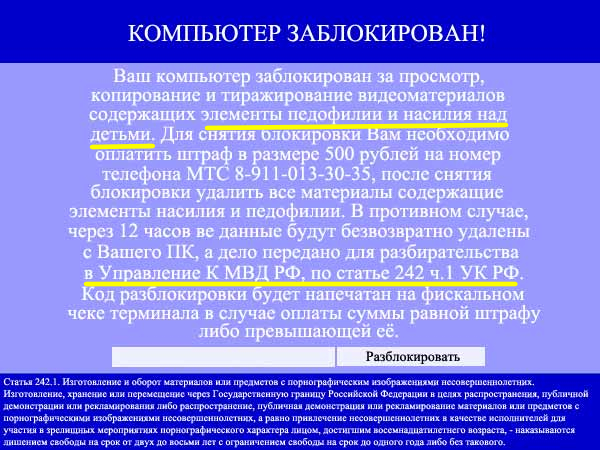
\includegraphics[width=0.8\textwidth]{images/winlocker2.jpg}}
\end{frame}

\section{Вирусы}
\subsection{Определение}
\begin{frame}
  \frametitle{Что такое \emph{вирус}?}
	\begin{itemize}[<+->]
	\item \emph{Компьютерный вирус} --- разновидность вредоносных компьютерных программ, отличительной особенностью которых является способность к размножению и/или самосохранению.
	\item В 1981 году Ричард Скрента написал один из первых загрузочных вирусов для Apple II — ELK CLONER. Он обнаруживал своё присутствие сообщением, содержащим небольшое стихотворение: \\
	\scriptsize{
    ELK CLONER:\\ 
    THE PROGRAM WITH A PERSONALITY\\
    IT WILL GET ON ALL YOUR DISKS\\
    IT WILL INFILTRATE YOUR CHIPS\\
    YES, IT'S CLONER\\
    IT WILL STICK TO YOU LIKE GLUE\\
    IT WILL MODIFY RAM, TOO\\
    SEND IN THE CLONER!\\}
	\end{itemize}
\end{frame}

\subsection{История}
\begin{frame}
  \frametitle{История вирусов}
	\begin{itemize}[<+->]
	  \item Первые вирусы зачастую не влияли глобально на работоспособность компьютера и/или сохранность информации.
	  \item Первый сетевой червь (\emph{червь Морриса}) появился в 1988 году. Задумывавшийся как безвредный, тем не менее, он причинил ущерба на сумму около 100.000.000\$.
	  \item Автор понёс наказание в виде 2 лет условно + 400 часов работ + 10.000\$.
	  \item Начиная с 1990 года вирусы приобрели характер глобальной эпидемии.
	\end{itemize}
\end{frame}

\subsection{Источник}
\begin{frame}
  \frametitle{Источник}
  
  \begin{enumerate}[<+->]
	  \item Накопители (USB флэшки, карты памяти, DVD/CD диски),
	  \item e-mail (картинки, объекты, архивы),
	  \item фишинг и социальный инжениринг,
	  \item Интернет (устаревшие браузеры, уязвимости в плагинах типа Flash, уязвимости в ОС, установка заражённых программ)
	\end{enumerate}
  
\end{frame}

\subsection{Фишинг}
\begin{frame}
  \frametitle{Пару слов о фишинге}
  \centerline{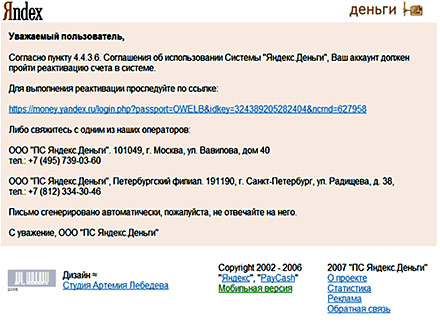
\includegraphics[width=0.8\textwidth]{images/fishing.jpg}}
\end{frame}

\subsection{Фишинг}
\begin{frame}
  \frametitle{Пару слов о фишинге}
  
  \begin{enumerate}[<+->]
	  \item Пользователям отправляется информация с просьбой зайти на определённый сайт и ввести данные.
	  \item Сайт может быть очень похож на реальный, включая дизайн и доменное имя (google.com vs gooogle.com).
	  \item Как вариант: злоумышленник может требовать отправить SMS / некоторую сумму \$ для активации / разблокировки и пр.
	  \item Рассылки могут быть направленными!
	  \item Вкупе с червями эффект увеличивается в разы.
	\end{enumerate}
  
\end{frame}

\section{Защита от вирусов}
\subsection{Условие}
\begin{frame}
  \frametitle{Необходимое условие}
  \centerline{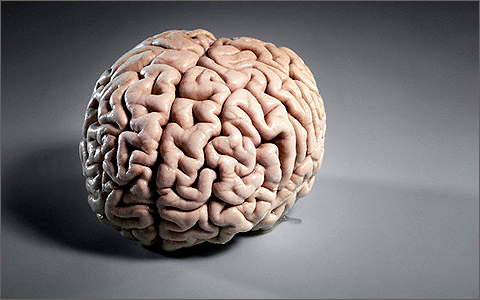
\includegraphics[width=0.8\textwidth]{images/brain.jpg}}
\end{frame}

\subsection{Народный метод}
\begin{frame}
  \frametitle{Советы народных целителей}
  \centerline{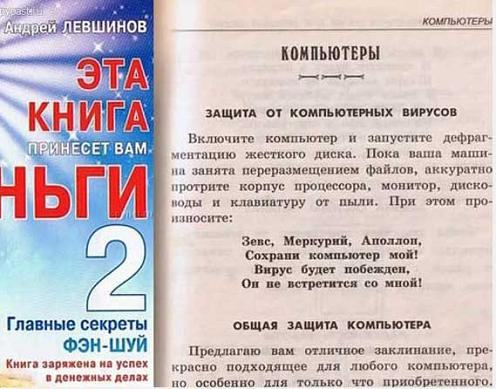
\includegraphics[width=0.8\textwidth]{images/magic.jpg}}
\end{frame}

\subsection{Кардинальный метод}
\begin{frame}
  \frametitle{Кардинальный метод}
  \centerline{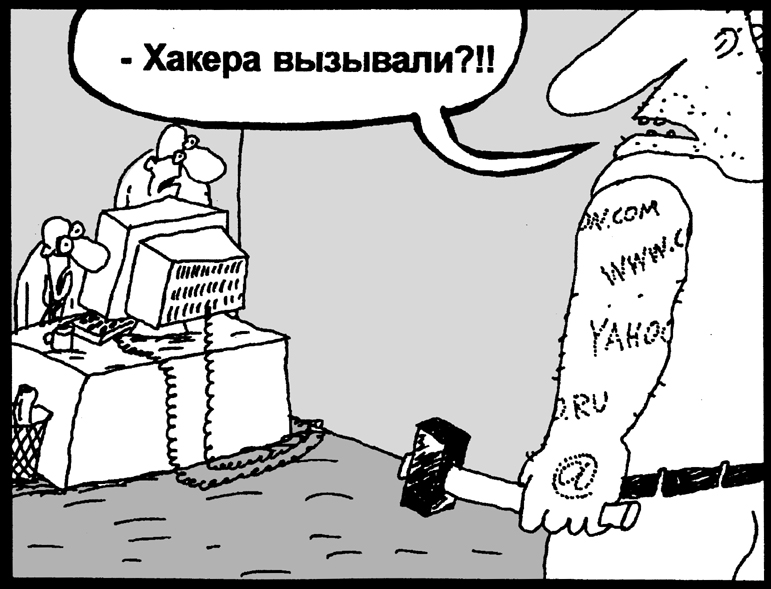
\includegraphics[width=0.8\textwidth]{images/WhatToDo.jpg}}
\end{frame}

\subsection{Реальный метод}
\begin{frame}
  \frametitle{Реальный метод}
  \begin{enumerate}[<+->]
    \item Делать только то, что понимаешь.
    \item Скачивать и устанавливать программы / контент с \textbf{проверенных} ресурсов.
    \item Постоянно (\textbf{каждый день!}) обновлять систему и ПО.
    \item Использовать антивирусы \textbf{И} файерволлы.
    \item Для сёрфинга использовать Firefox / Safari / Chrome с выключенными плагинами (типа Flash, Java и пр.).
    \item Перейти на Linux / Mac OS X
  \end{enumerate}
\end{frame}

\subsection{Реальный метод}
\begin{frame}
  \frametitle{Защита от фишинга и инженирии}
  \begin{enumerate}[<+->]
    \item Сначала думать, потом делать.
    \item Использовать сложные пароли, не хранить их в текстовых файлах / открытом виде.
    \item \textbf{Никогда} не вводить важные логины и пароли на ``левых'' сайтах. Только на известных.
    \item Понять, что халявы не бывает.
    \item Понять, что Дуров --- не идиот, и не будет вводить платные SMS-ки для школоты.
    \item При проблеме \textbf{сначала} посоветоваться с Google.
    \item Поднимать свой уровень знаний о компьютере.
  \end{enumerate}
\end{frame}

\section{Вместо эпилога}
\subsection{Видео}
\begin{frame}
  \frametitle{Mikko Hypponen}
  \begin{enumerate}[<+->]
    \item Директор антивирусной компании F-Secure.
    \item Офисы более чем в 100 странах.
    \item Home: mikko.hypponen.com.
    \item Twitter: @mikkohypponen.
    \item Беседа о вирусах.
    \item Short link: http://goo.gl/duqGk
  \end{enumerate}
\end{frame}

\subsection{}
\begin{frame}
  \frametitle{Будущее юных хакеров}
  \centerline{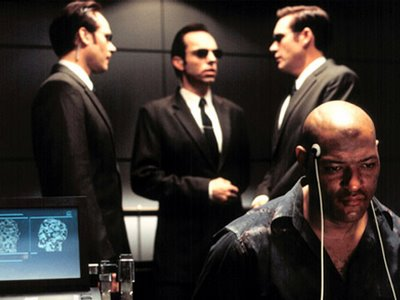
\includegraphics[width=0.8\textwidth]{images/HackerDestiny.jpg}}
\end{frame}


\section{Благодарности}
\begin{frame}
  \begin{itemize}
    \item Википедия (http://wikipedia.org),
    \item Google :),
    \item TED (http://ted.com),
    \item Множеству сайтов, которые распарсил Google, из которого были взяты замечательные картинки.
  \end{itemize}
\end{frame}

\end{document}